\chapter{Functies}
\label{cha:functies}
\thispagestyle{empty}


Als een programma langer wordt, dan wordt het al snel onoverzichtelijk.
Sommige stukken code komen misschien meerdere keren in het programma voor.
Bijvoorbeeld het inlezen van een positief getal.
Dit kopiëren van code zorgt ervoor dat het programma slecht onderhoudbaar wordt.
Als er namelijk een wijziging in deze code moet worden doorgevoerd dan moeten ook alle kopietjes worden aangepast. 
Ook zijn delen uit zo'n lang programma niet eenvoudig te gebruiken in een ander programma.
De code is slecht herbruikbaar.

We kunnen deze problemen oplossen door het gebruik van \textsl{functies}\index{functie}.
Een logisch bij elkaar behorend stuk code wordt dan ergens apart (in een functie) geplaatst.
Deze functie kunnen we vervolgens naar believen aanroepen om de code van de functie uit te voeren.


\newpage
\section{Een eenvoudige functie}
Als sterk versimpeld voorbeeld beschouwen we het programma dat gegeven is in listing~\ref{cod:slaregelsover1}.

%\floatlstinput[style=cstyle]{slaregelsover1.c}{slaregelsover1}{Een programma waar op wee plaatsen drie regels overgeslagen worden, zie \proglink{slaregelsover1.c}.} 

\booklisting[]{C}{Een programma waar op twee plaatsen drie regels overgeslagen worden}{slaregelsover1}{c}{!ht}


Op twee plaatsen in dit programma worden, in de uitvoer van het programma, drie regels overgeslagen.
In plaats van deze code te dupliceren kunnen we deze code ook opnemen in een functie.
Het is belangrijk om de functie een duidelijke naam te geven die aangeeft wat de functie doet.
In dit geval is gekozen voor de naam \texttt{sla\_3\_regels\_over}.
Het programma waarbij gebruikt gemaakt wordt van een functie is gegeven in \ref{cod:slaregelsover2}.



\booklisting[]{C}{Gebruik van de functie \texttt{sla\_3\_regels\_over}}{slaregelsover2}{c}{!ht}
%\floatlstinput[style=cstyle]{slaregelsover2.c}{slaregelsover2}{Een programma waar op twee plaatsen drie regels overgeslagen worden met behulp van de functie \ccode{sla_3_regels_over}, zie \proglink{slaregelsover2.c}.} 



Bovenin het programma wordt de functie \texttt{sla\_3\_regels\_over} gedefinieerd.
Het keyword \texttt{void}\indexkeyword{void} betekent leeg.
Het gebruik van \texttt{void} vóór de functienaam geeft aan dat deze functie niets teruggeeft.
Verderop in dit hoofdstuk zul je zien hoe een functie indien gewenst wel iets kan teruggeven.
Het gebruik van \texttt{void} na de functienaam, tussen de haken, geeft aan dat aan deze functie niets meegegeven kan worden bij aanroep. 
Verderop in dit hoofdstuk zullen we zien hoe aan een functie, indien gewenst, wel iets kan worden meegeven bij aanroep.
Vervolgens wordt deze functie in \texttt{main} twee maal aangeroepen met de code \texttt{sla\_3\_regels\_over()}.
De haakjes \texttt{()} achter de functienaam geven aan dat de functie aangeroepen moet worden.
 
Als dit programma gestart wordt, begint de uitvoering zoals gebruikelijk bij \texttt{main}.
Als de aanroep \texttt{sla\_3\_regels\_over()} moet worden uitgevoerd, wordt naar de code van deze functie gesprongen.
Aan het einde van de functie wordt teruggekeerd achter de plaats waar de functie is aangeroepen en wordt de uitvoering van het programma daar voortgezet.
Bij het aanroepen van een functie ``onthoudt'' de processor dus waarvandaan de functie aangeroepen wordt, zodat het programma na afloop van de functie na deze aanroep kan worden vervolgd.

De functie moet ``gezien'' zijn voordat de functie aangeroepen kan worden.
Vandaar dat de definitie van de functie \texttt{sla\_3\_regels\_over()} boven \texttt{main} geplaatst is.
Het is echter niet nodig om de volledige code van de functie voor \texttt{main} te definiëren.
Het is voldoende om alleen de eerste regel van de functie voor \texttt{main} te definiëren.
Dit wordt dan een \textsl{functiedeclaratie}\index{functiedeclaratie} of \textsl{functieprototype}\index{functieprototype} genoemd.
De volledige code van de functie moet natuurlijk nog wel worden gedefinieerd.
Dit kan bijvoorbeeld na \texttt{main} maar kan ook in een apart bestand.
We komen hier verderop in deze paragraaf op terug.

%TODO verwijzing toevoegen.
In listing~\ref{cod:slaregelsover3} kun je zien hoe je een functiedeclaratie kunt gebruiken\footnote{%
	Als je de functiedeclaratie vergeet zal het programma wel compileren, al zal de compiler wel een waarschuwing geven. 
	De compiler is in dit geval namelijk niet in staat om te controleren of de functie correct wordt aangeroepen. 
	Het is dus sterk aan te raden om als een functie niet boven \texttt{main} gedefinieerd is een functiedeclaratie te gebruiken. Overigens geeft Visual Studio standaard een foutmelding.
}.

%\floatlstinput[style=cstyle]{slaregelsover3.c}{slaregelsover3}{Een programma waarin een functiedeclaratie gebruikt is, zie \proglink{slaregelsover3.c}.} 
\booklisting[]{C}{Een programma waarin een functiedeclaratie gebruikt is.}{slaregelsover3}{c}{!ht} 

%\newcommand{\booklisting}[6][]{%
%\begin{figure}[#6]%
%\lstinputlisting[language=#2,caption={#3.},label=cod:#4,#1]{code/#4.#5}%
%\vspace*{-\baselineskip}
%\end{figure}%
%}


 
\section{Functies met parameters} 
Als een nog steeds sterk versimpeld voorbeeld beschouwen we nu het programma dat gegeven is in listing~\ref{cod:slaregelsover4}

%\floatlstinput[style=cstyle]{slaregelsover4.c}{slaregelsover4}{Een programma waar op twee plaatsen een aantal regels overgeslagen wordt, zie \proglink{slaregelsover4.c}.} 
\booklisting[]{C}{Een programma waar op twee plaatsen een aantal regels overgeslagen wordt}{slaregelsover4}{c}{!ht}

Op twee plaatsen in dit programma worden, in de uitvoer van het programma, regels overgeslagen.
De eerste keer worden drie regels overgeslagen en de tweede keer worden vier regels overgeslagen.
We kunnen nu een functie kunnen definiëren om drie regels over te slaan en nog een andere functie om vier regels over te slaan.
Maar het zou natuurlijk veel handiger zijn als we een functie zouden kunnen definiëren waarmee je een variabel aantal regels kunt overslaan.
Dit is mogelijk door een functie met een zogenoemde \textsl{parameter}\index{parameter} te definiëren.
Bij aanroep van de functie moet dan een zogenoemd \textsl{argument}\index{argument} worden meegegeven.
De waarde van het argument wordt dan bij aanroep van de functie naar de parameter gekopieerd.

In~\ref{cod:slaregelsover5} kun je zien hoe de functie \texttt{sla\_regel\_over} is gedefinieerd.
De functie heeft een parameter van het type \texttt{int}.
Bij de eerste aanroep van de functie wordt het argument \texttt{3} meegegeven.
Deze waarde wordt bij aanroep gekopieerd naar de parameter \texttt{aantal}.
Een parameter is in feite niets anders dan een variabele die bij het aanroepen van de functie geïnitialiseerd wordt met de waarde van het bij aanroep meegegeven argument.
De code van de functie wordt vervolgens uitgevoerd.
Doordat de parameter \texttt{aantal} is geïnitialiseerd met de waarde \texttt{3} wordt de code in de \texttt{for}-instructie drie maal herhaald en daardoor worden in de uitvoer drie regels overgeslagen.
De parameter \texttt{aantal} is alleen in de functie \texttt{sla\_regels\_over} te gebruiken.
Buiten de functie is de parameter onbekend.  
Bij de tweede aanroep van de functie wordt het argument \texttt{4} meegegeven.
Deze waarde wordt bij aanroep gekopieerd naar de parameter \texttt{aantal}.
De code van de functie wordt vervolgens weer uitgevoerd.
Doordat de parameter \texttt{aantal} nu is geïnitialiseerd met de waarde \texttt{4} wordt de code in de \texttt{for}-instructie vier maal herhaald en daardoor worden in de uitvoer vier regels overgeslagen.

%\floatlstinput[style=cstyle]{slaregelsover5.c}{slaregelsover5}{Een programma waar op twee plaatsen een aantal regels overgeslagen wordt met behulp van de functie \ccode{sla_regels_over}, zie \proglink{slaregelsover5.c}.} 
\booklisting[]{C}{Een programma waar op twee plaatsen een aantal regels overgeslagen wordt met behulp van de functie \texttt{sla\_regels\_over}}{slaregelsover5}{c}{!ht}


Een functie kan meerdere parameters hebben. 
De verschillende parameters worden van elkaar gescheiden door een komma.
Elke parameter heeft zijn eigen typeaanduiding.
Bij aanroep moet het aantal argumenten overeenkomen met het aantal parameters.
De waarde van het eerste argument wordt gekopieerd naar de eerste parameter en de waarde van het tweede argument wordt gekopieerd naar de tweede parameter enzovoort.



In listing~\ref{cod:print_rechthoek} is een voorbeeld gegeven van een functie met twee parameters.
De functie \texttt{print\_rechthoek} print een rechthoek met een bepaalde breedte en hoogte.
De uitvoer van het in~\ref{cod:print_rechthoek} gegeven programma is te zien in de onderstaande figuur.

%\floatlstinput[style=cstyle]{print_rechthoek.c}{print_rechthoek}{Een voorbeeld van een functie met twee parameters, zie \proglink{print_rechthoek.c}.} 

\booklisting[]{C}{Een voorbeeld van een functie met twee parameters}{print_rechthoek}{c}{!ht}


\begin{dosbox}
++++++++++++++++++++\\
+                  +\\
+                  +\\
+                  +\\
+                  +\\
+                  +\\
+                  +\\
++++++++++++++++++++
\end{dosbox}



De functie is bedoeld voor het tekenen van een rechthoek met een breedte groter dan 2 en kleiner dan 80 en een hoogte van groter dan 2 en kleiner dan 40. 
De standaardfunctie \texttt{assert}\indextwo{assert}{functie} wordt gebruikt om te controleren of de meegegeven argumenten aan deze voorwaarden voldoen.
Als de expressie die in de \texttt{assert} wordt gedefinieerd \texttt{false} oplevert, dan wordt het programma afgebroken en wordt een foutmelding gegeven.

Merk op dat de functie \texttt{print\_rechthoek} gebruik maakt van de functie \texttt{print\_lijn} om de boven- en onderkant van de rechthoek te printen.
De uitvoering van het programma start in \texttt{main}.
Vervolgens wordt de functie \texttt{print\_rechthoek} aangeroepen.
De terugkeerlocatie wordt ``onthouden'' door de processor door het ergens in het geheugen op te slaan.
Vervolgens wordt vanuit de functie \texttt{print\_rechthoek} de functie \texttt{print\_lijn} aangeroepen. 
Ook deze terugkeerlocatie wordt opgeslagen door de processor.

Na afloop van de functie \texttt{print\_lijn} wordt het programma vervolgt op de terugkeerlocatie die als laatste is opgeslagen.
Vervolgens wordt de \texttt{for}-instructie in \texttt{print\_rechthoek} uitgevoerd en daarna wordt \texttt{print\_lijn} nogmaals aangeroepen.
Ook deze terugkeerlocatie wordt weer opgeslagen door de processor.
Na afloop van de functie \texttt{print\_lijn} wordt het programma vervolgt op de terugkeerlocatie die zojuist is opgeslagen.
Na afloop van de functie \texttt{print\_rechthoek} wordt het programma vervolgd op de als eerste opgeslagen terugkeerlocatie.
De volgorde waarin terugkeerlocaties worden opgeslagen en weer worden opgeroepen wordt \textsl{LIFO}\index{lifo} (Last In First Out)\index{Last In First Out} genoemd.

\begin{infobox}[Stapelen maar...]
De processor slaat terugkeerlocaties op, op de zogenoemde \textsl{stack}\index{stack}. De bovenkant van de stack wordt aangewezen door een speciaal daarvoor bestemd register in de processor: de \textsl{stack pointer}\index{stack pointer}.
In figuur~\ref{fig:stack} is de stack getekend op het moment dat processor bezig is met het uitvoeren van de functie \texttt{print\_lijn}.

	\centering%
	\begin{tikzpicture}[scale=.8]
		\tikzset{>=latex}
		\tikzstyle{freecell}=[fill=infoboxbg,draw=black]
		\draw[freecell] (0, 0)
		+(-5.0,.5) -- +(-5.0,-.5) -- +(5.0,-.5) -- +(5.0,.5);
		\draw (0, 0) node{...};
		\draw[freecell] (0,-1) +(-5.0,-.5) rectangle +(5.0,+.5);
		\draw (0,-1) node {Terugkeerlocatie in \texttt{print\_rechthoek}};
		\draw[<-,line width=1pt] (0,-1) +(5.0,0) -- +(6.0,0);
		\draw (6.0,-1) node[anchor=west] {Stack Pointer};
		\draw[freecell] (0,-2) +(-5.0,-.5) rectangle +(5.0,+.5);
		\draw (0,-2) node {Terugkeerlocatie in \texttt{main}};
	\end{tikzpicture}
%	\caption{De stack op het moment dat de functie \texttt{print\_lijn} wordt uitgevoerd.}
%	\label{fig:stack}
\end{infobox}

\endinput

 
\subsection{Functies met een returnwaarde}
Tot nu toe heb je functies geschreven die iets afdrukken met behulp van |printf|.
Als je kijkt naar de standaard C-functie |sin| dan zie je dat deze functie niets afdrukt maar de sinus van het argument teruggeeft.
Een goed ontworpen functie moet in meerdere programma’s gebruikt kunnen worden.
Functies die het berekende resultaat meteen afdrukken zijn eigenlijk helemaal niet handig om te gebruiken in verschillende programma’s.
Stel je voor dat de functie |sin| de sinus van het argument meteen zou afdrukken in plaats van het resultaat terug te geven.
Deze functie zou dan slechts in een beperkt aantal gevallen te gebruiken zijn.
De versie die het resultaat teruggeeft is in veel meer gevallen te gebruiken. 
Soms zal de waarde van de sinus afgedrukt moeten worden, door de returnwaarde van de
|sin|-functie als argument door te geven aan de |printf|-functie:
\begin{clstfragment}
	print(sin(arg));
\end{clstfragment}
Maar meestal zal de waarde van de sinus gebruikt worden in een berekening:
\begin{clstfragment}
	overstaande_rechthoekszijde = sin(hoek) * schuine_zijde
\end{clstfragment}
De definitie van een C-functie die een waarde teruggeeft begint niet met |void| maar met het type van de waarde die wordt teruggegeven.
Dit wordt het returntype van de functie genoemd.
Vanuit de functie kan een waarde van het returntype worden teruggegeven met behulp van de |return|-instructie.
Er kan slechts één waarde worden teruggegeven via de |return|-instructie. 

In \cref{lst:gemiddelde1} is een voorbeeld gegeven van een functie die een waarde van het type |double| teruggeeft.
Deze functie berekent het gemiddelde van 3 als argumenten meegegeven gehele getallen.
  
\floatlstinput[style=cstyle]{gemiddelde1.c}{gemiddelde1}{Een eenvoudig voorbeeld van een functie met een returntype, zie \proglink{gemiddelde1.c}.}

De definitie van de functie |gemiddelde| begint met de typeaanduiding |double| waarmee aangegeven wordt dat deze functie een waarde van het type |double| teruggeeft.
In de functie wordt een |return|-statement gebruikt.
De waarde van de expressie achter |return| wordt gekopieerd naar de plaats waar de functie wordt aangeroepen.
De aanroep van de functie wordt als het ware vervangen door de returnwaarde.
In |main| wordt de waarde die wordt teruggegeven door de functie |gemiddelde| opgeslagen in de variabele |gem| en vervolgens afgedrukt met behulp van |printf|.

Er is in het voorbeeld dat is weergegeven in \cref{lst:gemiddelde1} gebruik gemaakt van de variabelen |resultaat| en |gem|, maar beide variabelen zijn in feite niet nodig.
In  \cref{lst:gemiddelde2} is een compactere versie van dit voorbeeld weergegeven.

\floatlstinput[style=cstyle]{gemiddelde2.c}{gemiddelde2}{Een compactere versie van het programma uit \cref{lst:gemiddelde1}, zie \proglink{gemiddelde2.c}.}

Een functie kan meerdere |return|-instructies bevatten. 
Zodra een |return|-in\-struc\-ties wordt uitgevoerd wordt de functie beëindigd.
Als eenvoudig voorbeeld is in \cref{lst:max1} een functie gegeven die de maximale waarde van twee, als argumenten meegegeven, gehele getallen teruggeeft.
Merk op dat je deze functie ook kan gebruiken om de maximale waarde van 3 getallen te bepalen door de returnwaarde van de ene aanroep te gebruiken als argument van de volgende aanroep.

\floatlstinput[style=cstyle]{max1.c}{max1}{Een programma dat drie gehele getallen inleest en de maximale waarde afdrukt, zie \proglink{max1.c}.}

Omdat de functie meteen wordt beëindigd als de return wordt uitgevoerd, is de |else| in de functie |max| overbodig. Zie \cref{lst:max2} voor een compactere versie van deze functie.

\floatlstinput[style=cstyle,linerange={3-10}]{max2.c}{max2}{Een compactere versie van de functie \ccode{max}, zie \proglink{max2.c}.}

Tot nu toe waren de functies die we als voorbeeld hebben bekeken nog niet zo heel goed bruikbaar in de praktijk.
Daarom sluiten we deze paragraaf af met een functie die je wel degelijk in de praktijk zou kunnen toepassen.
De uitvoer van het in \cref{lst:lees_geheel_getal} gegeven programma is te zien in \cref{fig:lees_geheel_getal}.
De door de gebruiker ingetypte invoer is groen en onderstreept weergegeven. 
In \cref{lst:lees_geheel_getal} is een functie gegeven die een geheel getal inleest, controleert of de ingevoerde waarde een getal is en of deze waarde tussen een als argument meegegeven minimale en maximale waarde ligt (inclusief).
Zolang dit niet zo is, wordt een foutmelding gegeven en kan de gebruiker het opnieuw proberen,

\floatlstinput[style=cstyle]{lees_geheel_getal.c}{lees_geheel_getal}{Een functie om een geheel getal in te lezen, zie \proglink{lees_geheel_getal.c}.}

\begin{myFigure}[!htbp]
	\centering%
	\begin{coutput}
Geef een geheel getal [1..10]: \cinput{0}
Onjuiste invoer. Probeer het opnieuw!
Geef een geheel getal [1..10]: \cinput{11}
Onjuiste invoer. Probeer het opnieuw!
Geef een geheel getal [1..10]: \cinput{zeven}
Onjuiste invoer. Probeer het opnieuw!
Geef een geheel getal [1..10]: \cinput{7}
Het ingelezen toetscijfer is 7.
	\end{coutput}
	\caption{Een mogelijke uitvoer van het programma uit \cref{lst:lees_geheel_getal}.}
	\label{fig:lees_geheel_getal}
\end{myFigure}

\subsection{Functies die meer dan één waarde teruggeven}
Met behulp van de |return|-instructie kun je in C vanuit een functie één waarde teruggeven.
Als je meerdere waarden wilt teruggeven dan kan dat op twee manieren.
\needspace{2cm}%
Je kunt:
\begin{itemize}
	\item
	de waarden \squote{inpakken} in een structure, dit wordt verderop in dit \MakeLowercase\documenttype{} behandeld, zie \cref{sec:struct};
	\item
	de waarden teruggeven via zogenoemde \emph{call by reference} parameters.
\end{itemize}

Bij het gebruik van normale parameters wordt de \emph{waarde} van elk argument gekopieerd naar de overeenkomstige parameter. Deze parameters worden ook wel \emph{call by value} parameters genoemd.
Call by reference parameters kunnen in C geimplementeerd worden door pointers, zie \cref{sec:pointers}, te gebruiken.
Beschouw het programma dat gegeven is in \cref{lst:foute_wissel}.
Het is de bedoeling dat de waarden van de variabelen x en y verwisseld zijn na aanroep van de functie |wissel(x, y)|.
Zo'n functie die twee getallen verwisseld kan bijvoorbeeld handig zijn bij het sorteren van getallen.
De uitvoer van dit programma is gegeven in \cref{fig:foute_wissel}.

Zoals je ziet zijn de waarden van de variabelen x en y \emph{niet} verwisseld na aanroep van de functie |wissel(x, y)|.
Dit hadden we natuurlijk kunnen zien aankomen.
Bij aanroep van de functie |wissel| wordt de waarde van de als argument meegegeven variabele |x| gekopieerd naar de parameter |a| en wordt de waarde van de als argument meegegeven variabele |y| gekopieerd naar de parameter |b|.
Vervolgens worden de waarden van |a| en |b| keurig verwisseld in de functie |wissel|, maar bij terugkeer in |main| hebben |x| en |y| nog steeds hun oorspronkelijke waarden.
De standaard parameteroverdacht in C is namelijk call by value.
Bij aanroep wordt de waarde van elk argument gekopieerd naar de bijbehorende parameter.    

\floatlstinput[style=cstyle]{foute_wissel.c}{foute_wissel}{Een \emph{niet werkende} functie om  twee getallen te verwisselen, zie \proglink{foute_wissel.c}.}

\begin{myFigure}[!htbp]
	\centering%
	\begin{coutput}
x = 7 en y = 8
x = 7 en y = 8
	\end{coutput}
	\caption{De uitvoer van het programma uit \cref{lst:foute_wissel}.}
	\label{fig:foute_wissel}
\end{myFigure}

Om de functie correct te laten functioneren moet je gebruik maken van pointers, zie \cref{lst:wissel}.
De uitvoer van dit programma is gegeven in \cref{fig:wissel}.
Als parameters van de functie |wissel| zijn nu twee pointers naar |int|'s gedefinieerd.
Bij aanroep van de functie wordt het adres van de variabele |x| als eerste argument meegegeven.
De waarde van dit adres wordt gekopieerd naar de parameter |ptr_a|.
Deze pointer \squote{wijst} of \squote{refereert} dus naar de variabele |x|.
Het adres van de variabele |y| wordt als tweede argument meegegeven.
De waarde van dit adres wordt gekopieerd naar de parameter |ptr_b|.
Deze pointer wijst dus naar de variabele |y|.

Bij aanvang van de functie |wissel| wordt de waarde van de variabele |hulpje| gelijk aan waarde waar de pointer |a_ptr| naar wijst.
Deze pointer wijst naar de variabele |x| en die heeft de waarde |7|, dus |hulpje| krijgt de waarde |7|.
Vervolgens wordt de variabele waar de pointer |a_ptr| naar wijst gelijk gemaakt aan de waarde waar de pointer |b_ptr| naar wijst.
|a_ptr| wijst naar de variabele |x| en |b_ptr| wijst naar de variabele |y|, die de waarde |8| heeft.
Dus |x| krijgt de waarde |8|.
Tot slot wordt de variabele waar de pointer |b_ptr| naar wijst gelijk gemaakt aan de waarde van de variabele |hulpje|.
|a_ptr| wijst naar de variabele |y| en |hulpje| heeft de waarde |7|.
Dus |y| krijgt de waarde |7|.
Bij terugkeer in |main| zijn waarden van de variabelen |x| en |y| dus inderdaad verwisseld, zoals de bedoeling was.

Het doorgeven van adressen als argumenten in plaats van waarden wordt call by reference genoemd.
Een adres refereert (verwijst) namelijk naar een bepaalde variabele in het geheugen en we geven de referentie naar de variabele door in plaats van de waarde van de variabele.

\floatlstinput[style=cstyle]{wissel.c}{wissel}{Een \emph{werkende} functie om  twee getallen te verwisselen, zie \proglink{wissel.c}.}

\begin{myFigure}[!htbp]
	\centering%
	\begin{coutput}
x = 7 en y = 8
x = 8 en y = 7
	\end{coutput}
	\caption{De uitvoer van het programma uit \cref{lst:wissel}.}
	\label{fig:wissel}
\end{myFigure}

%TODO voorbeeld berekenen reeele wortels van een kwadratische vergelijking. Verwijzen is waarschijnlijk beter! 

\subsection{Zichtbaarheid en levensduur van lokale variabelen}
\emph{Wordt nog aan gewerkt!}

|static|

\subsection{Recursieve functies}
Een functie die \emph{zichzelf} aanroept wordt een recursieve functie genoemd.
Een veel gebruikt voorbeeld van een toepassing van een recursieve functie is het berekenen van de faculteit van een natuurlijk getal $n$.
De faculteit van $n$ is gedefinieerd zoals gegeven in \cref{eq:fac}.
\begin{equation}
\label{eq:fac}
	n! = \prod_{i=1}^{n} i = 1 \cdot{} 2 \cdot{} 3 \cdot{} \cdots{} \cdot{} n
\end{equation} 
Dus bijvoorbeeld $4! = 1 \cdot{} 2 \cdot{} 3 \cdot 4 = 24$.
Verder is afgesproken: $0! = 1$.
Deze wiskundige functie is ook recursief te definiëren\footnote{%
	In een recursieve definitie wordt hetgeen gedefinieerd wordt in de definitie zelf gebruikt.
}, zie \cref{eq:fac_rec}.
\begin{equation}
\label{eq:fac_rec}
	n! =
	\begin{cases}
		1, & \text{als $n <= 1$}\\
		n \cdot{} (n - 1)!, & \text{als $n > 1$}
	\end{cases}
\end{equation} 
Dus $4!$ kan ook als volgt berekend worden: $4! = 4 \cdot{} 3! = 4 \cdot{} 3 \cdot{} 2! = 4 \cdot{} 3 \cdot{} 2 \cdot 1! = 4 \cdot{} 3 \cdot{} 2 \cdot 1 = 24.$

Als we deze recursieve definitie coderen in C krijgen we een recursieve functie, zie \cref{lst:faculteit_recursief}.

\floatlstinput[style=cstyle]{faculteit_recursief.c}{faculteit_recursief}{Een \emph{recursieve} functie om de faculteit van een natuurlijk getal te berekenen, zie \proglink{faculteit_recursief.c}.}

Omdat de faculteit gedefinieerd is voor natuurlijke getallen (gehele getallen groter dan of gelijk aan nul) is als type van de parameter |unsigned int| gekozen (een geheel getal zonder teken).
Omdat de waarde van de facuteit van grotere getallen al snel erg groot wordt, is als returntype het type |double| gekozen. De waarde van $13!$ past bijvoorbeeld al niet meer in een (32-bits) |unsigned int|. De waarde van $171!$ past ook al niet meer in een |double|. Het nadeel van het gebruik van |double| als returntype is dat de nauwkeurigheid van een |double| beperkt is tot ongeveer 17 significante cijfers\footnote{%
	De exacte waarde van $23! = 25852016738884976640000$ maar de functies uit \cref{lst:faculteit_recursief} geeft als resultaat 25852016738884978212864. Je ziet dat de eerste 16 cijfers correct zijn, de laatste 7 cijfers zijn echter niet juist. De functies geven dus slecht een benadering van $n!$ voor grotere waarden van $n$.  
}.

Het is in dit geval echter helemaal niet nodig om een recursieve functie te gebruiken.
Je kunt ook \squote{gewoon} een herhalings-instructie gebruiken om $n!$ te berekenen, zie \cref{lst:faculteit_iteratief}. Een functie die een herhalings-instructie gebruikt wordt, met een mooi woord, een \emph{iteratieve} functie genoemd. 
De meeste mensen zullen de code uit \cref{lst:faculteit_iteratief} eenvoudiger te begrijpen vinden dan de code uit \cref{lst:faculteit_recursief}. 

\floatlstinput[style=cstyle]{faculteit_iteratief.c}{faculteit_iteratief}{Een \emph{iteratieve} functie om de faculteit van een natuurlijk getal te berekenen, zie \proglink{faculteit_iteratief.c}.}

Een recursieve aanpak is vooral handig als er nog code wordt uitgevoerd \emph{na} de recursieve aanroep.
Stel dat je een natuurlijk getal wilt afdrukken in het elftallig stelsel\footnote{%
	Het elftallig stelsel is een positioneel talstelsel met elf als grondtal. Dit stelsel kent de cijfers 0 t/m 9 en A. Het getal 2A9 in het elftallig stelsel komt overeen met het getal $2 \times{} 11^2 + 10 \times{} 11 + 9 = 361$ in het tientallig stelsel. Het elftallig stelsel zou met Carnaval van pas kunnen komen, zie \url{https://www.telegraaf.nl/nieuws/1037460/gek-getal}.
}, dan kun je gebruik maken van het iteratieve algoritme dat gegeven is in \cref{fig:elftallig_iteratief}.

\figuur{scale=.7}{elftallig_iteratief}{Een iteratief algoritme om een getal om te zetten naar het elftallig stelsel.}

Als je het getal 361 met behulp van dit algoritme omzet naar het elftallig stelsel, dan produceert dit algoritme de uitvoer die is gegeven in \cref{fig:output_elftallig_iteratief}. 

\begin{myFigure}[!htbp]
	\centering%
	\begin{coutput}
cijfer op positie 0 = 9
cijfer op positie 1 = A
cijfer op positie 2 = 2
	\end{coutput}
	\caption{De uitvoer van het algoritme uit \cref{fig:elftallig_iteratief} als getal gelijk is aan 361.}
	\label{fig:output_elftallig_iteratief}
\end{myFigure}

Als we echter het elftallige resultaat op de normale manier willen afdrukken als |2A9|, dan is dat lastig omdat de cijfers in de verkeerde volgorde worden gegenereerd door het iteratieve algoritme.
Je moet dus de gegenereerde cijfers ergens opslaan en ze aan het einde in de omgekeerde volgorde afdrukken.
Dit zou je kunnen doen door een zogenoemde array te gebruiken, zie \cref{sec:arrays} verderop in dit \MakeLowercase\documenttype{}. 
Maar je zou ook gebruik kunnen maken van het recursieve algoritme dat gegeven is in \cref{fig:elftallig_recursief}
 
\figuur{scale=.55}{elftallig_recursief}{Een recursief algoritme om een getal om te zetten naar het elftallig stelsel.}

\newcommand{\printInElftalligStelsel}{\hcode{print\\-In\\-Elf\\-tal\\-lig\\-Stel\\-sel}}

We maken in dit geval slim gebruik van het feit dat functies die achtereenvolgens aangeroepen worden in de omgekeerde volgorde terugkeren (LIFO, zie \cpageref{lifo}).
Als we ervan uitgaan dat het argument dat wordt doorgegeven aan de functie \printInElftalligStelsel{} voorafgaande aan de functieaanroep op de stack wordt gezet, dan ziet de stack er nadat de functie voor de derde keer is aangeroepen uit zoals gegeven in \cref{fig:stackelftallig}.

\begin{myFigure}
	\centering%
	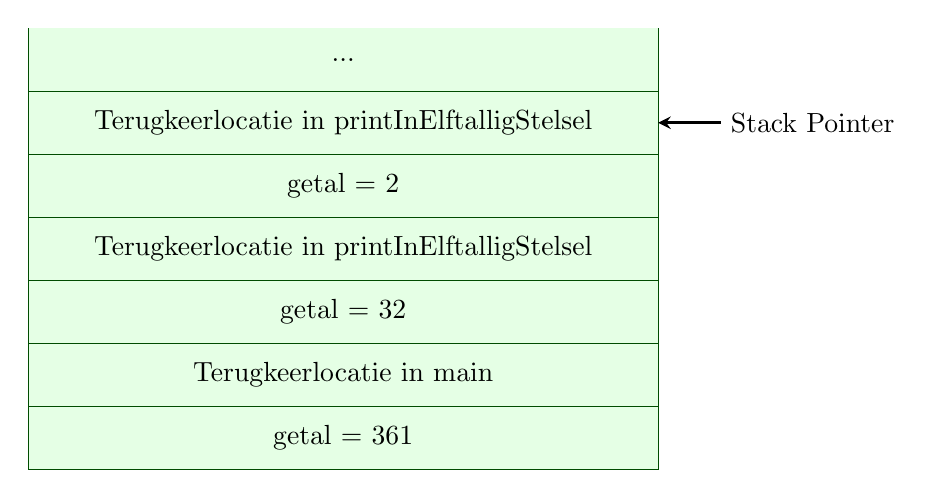
\begin{tikzpicture}[scale=.8]
	\tikzset{>=stealth}
	\tikzstyle{freecell}=[fill=green!10,draw=green!30!black]
	\draw[freecell] (0, 0)
	+(-5,.5) -- +(-5,-.5) -- +(5,-.5) -- +(5,.5);
	\draw (0, 0) node{...};
	\draw[freecell] (0,-1) +(-5,-.5) rectangle +(5,+.5);
	\draw (0,-1) node {Terugkeerlocatie in \ccode{printInElftalligStelsel}};
	\draw[<-,line width=1pt] (0,-1) +(5,0) -- +(6,0);
	\draw (6,-1) node[anchor=west] {Stack Pointer};
	\draw[freecell] (0,-2) +(-5,-.5) rectangle +(5,+.5);
	\draw (0,-2) node {\ccode{getal = 2}};
	\draw[freecell] (0,-3) +(-5,-.5) rectangle +(5,+.5);
	\draw (0,-3) node {Terugkeerlocatie in \ccode{printInElftalligStelsel}};
	\draw[freecell] (0,-4) +(-5,-.5) rectangle +(5,+.5);
	\draw (0,-4) node {\ccode{getal = 32}};
	\draw[freecell] (0,-5) +(-5,-.5) rectangle +(5,+.5);
	\draw (0,-5) node {Terugkeerlocatie in \ccode{main}};
	\draw[freecell] (0,-6) +(-5,-.5) rectangle +(5,+.5);
	\draw (0,-6) node {\ccode{getal = 361}};
	\end{tikzpicture}
	\caption{De stack op het moment dat de functie \printInElftalligStelsel{} drie maal is aangeroepen.}
	\label{fig:stackelftallig}
\end{myFigure}

De implementatie in de programmeertaal C van het algoritme gegeven in \cref{fig:elftallig_recursief} is gegeven in \cref{lst:elftallig_recursief}

\floatlstinput[style=cstyle]{elftallig_recursief.c}{elftallig_recursief}{De implementatie in de programmeertaal C van het in \cref{fig:elftallig_recursief} gegeven algoritme, zie \proglink{elftallig_recursief.c}.} 

Omdat het erg belangrijk is dat je goed begrijpt hoe dit programma door de processor wordt uitgevoerd, wordt dit hier stap voor stap besproken.
In de functie |main| wordt de functie \printInElftalligStelsel{} aangeroepen met als argument |361|. 
Deze waarde wordt op de stack geplaatst en daarna wordt naar de code van de functie gesprongen. Het terugkeeradres in |main| wordt op de stack geplaatst (bovenop de waarde |361|).
In de functie wordt de plaats op de stack waar de waarde van het argument is geplaatst aangeduid met de variabelenaam |getal|.
Omdat de waarde van |getal| groter is dan 11 wordt de functie \printInElftalligStelsel{} nogmaals aangeroepen, nu moet |getal / 11| als argument.
|getal| heeft de waarde |361| dus de waarde van het argument is |361 / 11| = |32|.
Deze waarde wordt op de stack geplaatst en daarna wordt naar de code van de functie gesprongen. Het terugkeeradres in \printInElftalligStelsel{} wordt op de stack geplaatst (bovenop de waarde |32|).
In de functie wordt de plaats op de stack waar de waarde van het argument is geplaatst aangeduid met de variabelenaam |getal|.
Omdat de waarde van |getal| groter is dan 11 wordt de functie \printInElftalligStelsel{} nogmaals aangeroepen, nu moet |getal / 11| als argument.
|getal| heeft de waarde |32| dus de waarde van het argument is |32 / 11| = |2|.
Het terugkeeradres in \printInElftalligStelsel{} wordt op de stack geplaatst (bovenop de waarde |2|).
De inhoud van de stack is nu weergegeven in \cref{fig:stackelftallig}.

De functie \printInElftalligStelsel{} wordt nu niet meer aangeroepen.
De variabele |cijfer| wordt aangemaakt en krijgt de waarde |getal % 11|.
|getal| heeft de waarde |2| dus cijfer krijgt de waarde |2|, dit cijfer wordt vervolgens afgedrukt.
Aan het einde van de functie \printInElftalligStelsel{} wordt het terugkeeradres en het argument van de stack verwijderd.
We keren dus terug naar de plaats waar \printInElftalligStelsel{} in \printInElftalligStelsel{} is aangeroepen en dat is het einde van de |if|-instructie.
De variabele |getal| heeft in deze functie de waarde |32|.
De variabele |cijfer| wordt aangemaakt en krijgt de waarde |getal % 11|.
|getal| heeft de waarde |32| dus cijfer krijgt de waarde |10|, vervolgens wordt het \squote{cijfer} |A| afgedrukt.
Aan het einde van de functie \hcode{print\\-In\\-Elf\\-tal\\-lig\\-Stel\\-sel} wordt het terugkeeradres en het argument van de stack verwijderd.
We keren dus terug naar de plaats waar \printInElftalligStelsel{} in \printInElftalligStelsel{} is aangeroepen en dat is het einde van de |if|-instructie.
De variabele |getal| heeft in deze functie de waarde |361|.
De variabele |cijfer| wordt aangemaakt en krijgt de waarde |getal % 11|.
|getal| heeft de waarde |361| dus cijfer krijgt de waarde |9|, dit cijfer wordt vervolgens afgedrukt.
Aan het einde van de functie \printInElftalligStelsel{} wordt het terugkeeradres en het argument van de stack verwijderd.
We keren dus terug naar de plaats waar \printInElftalligStelsel{} in |main| is aangeroepen en het programma wordt beëindigd.

In \cref{lst:print_in_talstelsel} is een soortgelijk voorbeeld gegeven van een recursieve functie met twee parameters.
De functie |print_in_talstelsel| zal de integer (zonder teken) die als eerste argument wordt meegegeven afdrukken in het als tweede argument meegegeven talstelsel.
De uitvoer van het in \cref{lst:print_in_talstelsel} gegeven programma is te zien in \cref{fig:print_in_talstelsel}.

\floatlstinput[style=cstyle]{print_in_talstelsel.c}{print_in_talstelsel}{Een voorbeeld van een recursieve functie, zie \proglink{print_in_talstelsel.c}.} 

\begin{myFigure}[!htbp]
	\centering%
	\begin{coutput}
1111101000
2626
1000
3E8
CAFE
	\end{coutput}
	\caption{De uitvoer van het programma uit \cref{lst:print_in_talstelsel}.}
	\label{fig:print_in_talstelsel}
\end{myFigure}

Twee andere leerzame toepassingen van recursieve functies zijn:
\begin{itemize}
	\item
	Een programma dat sudoku's op kan lossen:
	\iftoggle{ebook}{%
		\href{https://bitbucket.org/HR_ELEKTRO/cpl01/downloads/sudokuEbook.pdf}{sudokuEbook.pdf}%
	}{
		\href{https://bitbucket.org/HR_ELEKTRO/cpl01/downloads/sudoku.pdf}{sudoku.pdf}%
	}
    \item
    Een programma dat Boter Kaas en Eieren kan spelen:  
	\iftoggle{ebook}{%
		\href{https://bitbucket.org/HarryBroeders/dictaat-algoritmen-en-datastructuren-in-c99/downloads/Tic-Tac-Toe_ebook.pdf}{Tic-Tac-Toe\_ebook.pdf}%
	}{
		\href{https://bitbucket.org/HarryBroeders/dictaat-algoritmen-en-datastructuren-in-c99/downloads/Tic-Tac-Toe.pdf}{Tic-Tac-Toe.pdf}%
	}
\end{itemize}

\subsection{Functie als parameter}
%TODO functie als parameters
\emph{Wordt nog aan gewerkt!}

\subsection{Programma verdelen over meerdere bestanden}
\emph{Wordt nog aan gewerkt!}
